\documentclass[10pt]{article}

\usepackage[margin=0.75in]{geometry}
\usepackage{amsmath,amsthm,amssymb}
\usepackage{xcolor}
\usepackage{cancel}
\usepackage{graphicx}
\usepackage{changepage}
\usepackage{circuitikz}
\usepackage{pgfplots}
\usepackage{physics}
\usepackage{hyperref}
\usepackage{minted}
\usepackage[breakable]{tcolorbox}
\usepackage[inline]{enumitem}

\theoremstyle{definition}
\newtheorem{problem}{Problem}
\newtheorem{soln}{Solution}

\pgfplotsset{compat=newest}
\usetikzlibrary{lindenmayersystems}
\usetikzlibrary{arrows}

\definecolor{incolor}{HTML}{303F9F}
\definecolor{outcolor}{HTML}{D84315}
\definecolor{cellborder}{HTML}{CFCFCF}
\definecolor{cellbackground}{HTML}{F7F7F7}
\newcommand{\eq}{=}
\tikzset
{%
  axes/.style={thick,-latex},
  cylinder/.style={right color=blue!80,left color=white,fill opacity=0.7},
  paraboloid back/.style={left color=magenta!80,fill opacity=0.4},
  paraboloid front/.style={left color=white, right color=magenta!80,fill opacity=0.4},
}

\makeatletter
\newcommand{\boxspacing}{\kern\kvtcb@left@rule\kern\kvtcb@boxsep}
\makeatother
\newcommand{\prompt}[4]{
    \ttfamily\llap{{\color{#2}[#3]:\hspace{3pt}#4}}\vspace{-\baselineskip}
}

\newcommand{\highlight}[1]{\colorbox{yellow}{$\displaystyle #1$}}

\newcommand{\volts}[0]{\mathrm{V}}
\newcommand{\amps}[0]{\mathrm{A}}
\newcommand{\ohms}[0]{\Omega}
\newcommand{\farad}[0]{\mathrm{F}}
\newcommand{\coulomb}[0]{\mathrm{C}}
\newcommand{\watts}[0]{\mathrm{W}}

\hypersetup{
    colorlinks=true,
    linkcolor=blue,
    filecolor=magenta,      
    urlcolor=cyan,
    pdftitle={Overleaf Example},
    pdfpagemode=FullScreen,
    }

\NewDocumentCommand{\evalat}{sO{\big}mm}{%
  \IfBooleanTF{#1}
   {\mleft. #3 \mright|_{#4}}
   {#3#2|_{#4}}%
}

\title{Physics 2130: Lab 2B}
\author{Jeremy Favro}
\date{\today}

\begin{document}

\maketitle

\inputminted{python}{lab2b.py}
\newpage
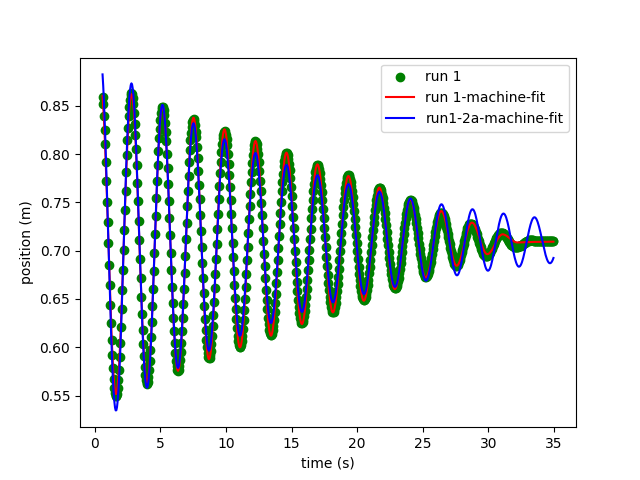
\includegraphics{Figure_0.png}\\
The model incorporating friction appears to (and does per the residuals) fit this data better than last week's model. \\
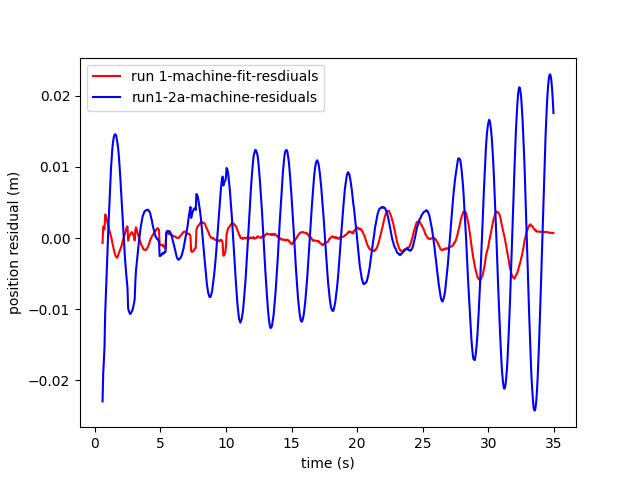
\includegraphics{Figure_99-R1R.png}\\
As seen on the graph this model is a much better fit compared to last week's for this data. In this case this is true effectively everywhere.

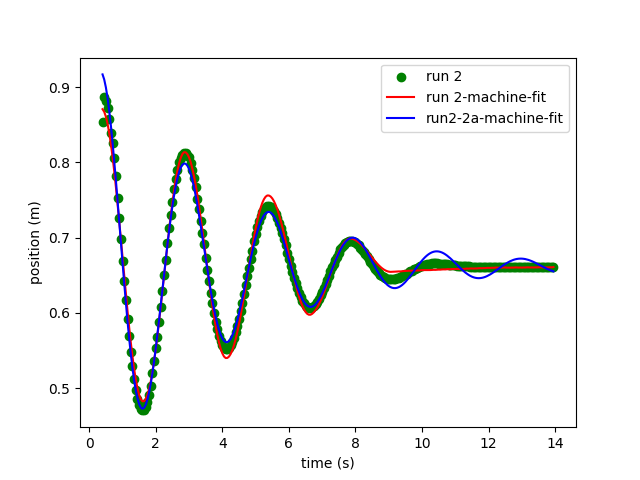
\includegraphics{Figure_1.png}\\
In this case both models seem to fail in different ways. This week's model overestimates the actual value, whereas last week's underestimated it.
Near the end ($t\to t_f$) this week's model is a definite better fit as it actually reaches $\approx x_{eq}$. \\
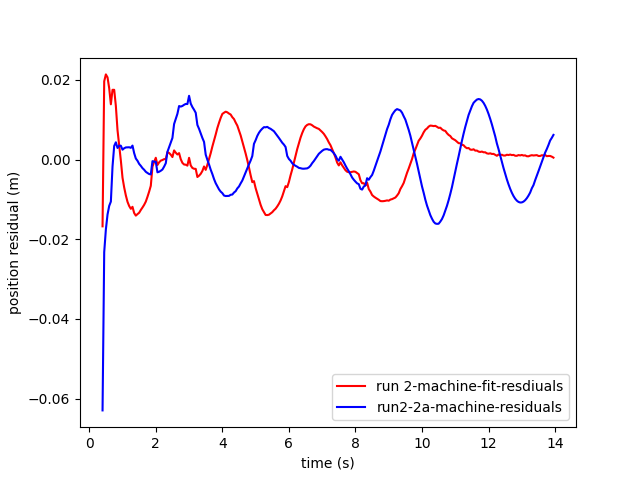
\includegraphics{Figure_100-R2R.png}\\
As seen on the graph last week's model underestimates whereas last week's overestimates. Also as seen on the graph this week's 
model does a much better job at fitting the data near the end where the real data has decayed.
\newpage

\inputminted{python}{lab2b-ex.py}
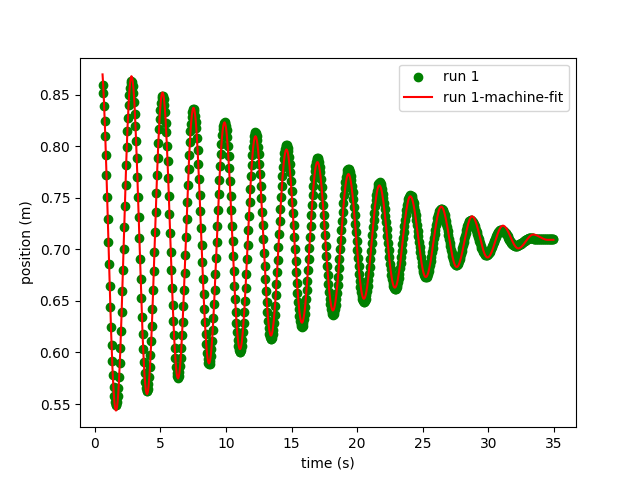
\includegraphics{Figure_0-N.png}\\
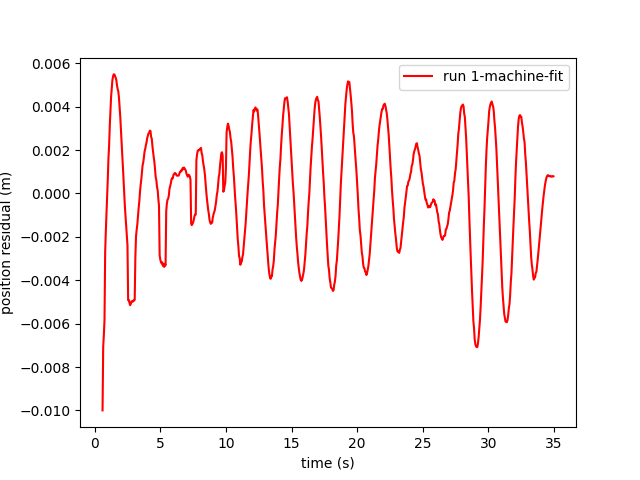
\includegraphics{Figure_10-R1RN.png}\\
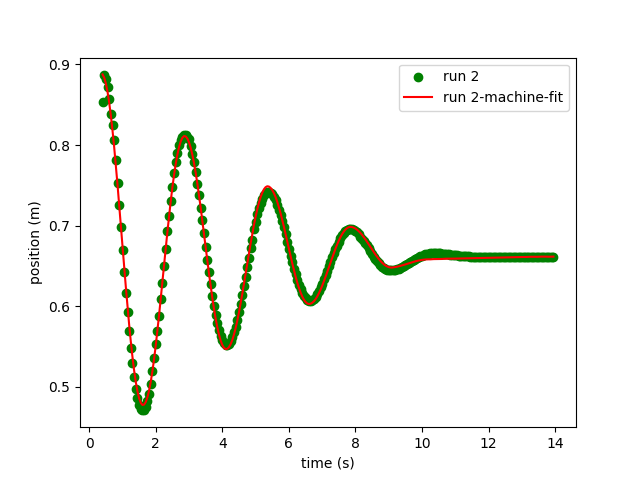
\includegraphics{Figure_1-N.png}\\
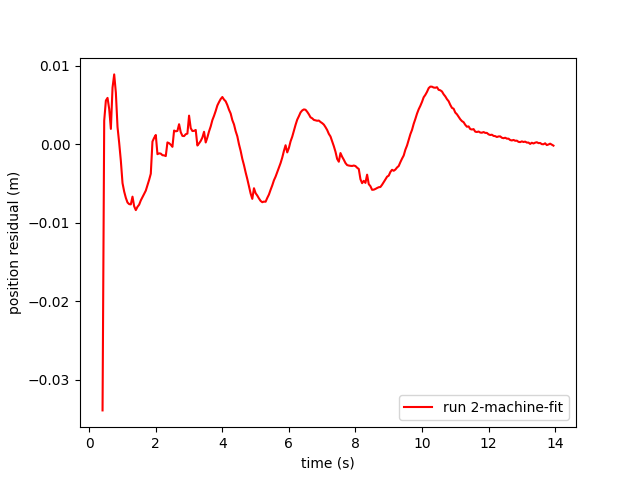
\includegraphics{Figure_11-R2RN.png}\\

Given the significant decrease in the residuals the first run and the slight improvement in run 2 I would say that the effort to change the model is definitely worth it.
\end{document}